% !TEX root = thesis-main.tex


\chapter{Topic-Sensitive Word Representations}
\label{chapter:research-01}

\section{Introduction and research questions}


Word representations in the form of dense vectors, or word embeddings, capture semantic and syntactic information \citep{mikolov2013efficient,pennington2014glove} and are widely used in many NLP tasks such as sentiment analysis \citep{tang2014learning,yu-etal-2017-refining}, identifying multiword expressions \citep{salehi-etal-2015-word,gharbieh2016word}, and translation \citep{zou2013bilingual, artetxe-etal-2018-unsupervised}.
These representation models are based on the assumption that the meaning of a word can be inferred from its textual context \citep{firth1957synopsis}. 

Currently, there are two categories of approaches to learning word representations (discussed in Section~\ref{bgemb}): \textit{static embeddings} where a fixed vector is learned for each word in the vocabulary, and \textit{dynamic embeddings} where vectors are dynamically calculated for each sentence. 
Dynamic embeddings such as ELMo \citep{peters-etal-2018-deep} and BERT \citep{devlin-etal-2019-bert} store the learned weights of the network, and use that to get word representations by computing them on the fly for a given context.
As a result, these models can capture context-dependent characteristics of the language such as polysemy: in natural language, words usually have more than one meaning (or sense).

%While these models perform extremely well on several NLP tasks, they are computationally expensive to acquire and use. 
%Static embeddings, on the other hand, are cost-effective and instantly accessible for nearly all downstream tasks.
Like dynamic embeddings, the research presented in this chapter aims at overcoming the inability of static embeddings to capture polysemy.
However, it predates dynamic embeddings.
Before the advent of contextualized embedding approaches, most static representation models learned \textit{one} fixed-length representation per word. 
However, this approach and how it is evaluated has some shortcomings.

Firstly, many tasks can benefit from using multiple representations per word to capture polysemy \citep{Bengio:2003,reisinger-mooney:2010:NAACLHLT}.
Many intricate distinctions of word senses are lost when we use one embedding vector to capture multiple meanings.
Additionally, this simplification of natural language unintentionally leads to more simplistic evaluation tasks.  
Most studies on static word embeddings used word similarity task to assess the accuracy of the static word representations where word pairs are ranked based on how similar or related they are.
However, most of the word similarity benchmarks present words out of context. The word pair `\textit{bank}' and `\textit{reef}' can have very different similarity scores depending on the context of the word \textit{bank}.
Finally, there is no clear and quantifiable definition of \textit{similarity} and \textit{relatedness} when comparing two words, and as a result, different benchmarks have different interpretations \citep{faruqui2016problems}. 

In this chapter, we seek to address these shortcomings and propose an approach for learning multiple static word representations per word.
We aim to understand the role of a particular kind of context, namely document topics, for learning these representations.
We analyze to what extent learning multiple topic-sensitive embeddings per word captures polysemy, which we believe is a necessary step towards further understanding the impact of context. 
Concretely, we ask: 


\paragraph{Research Question 1:} \acl{rq:topic} 

\medskip

 \noindent We first look at the importance of document-level context and how it can help to separate different meanings of the word.
We study the integration of this topical information in learning word representation and evaluate the embeddings on a contextual task. 
Concretely, we ask: 
 
\begin{enumerate}[label=\textbf{RQ1.\arabic* },wide = 0pt, leftmargin=2em]
\setlength\itemsep{1em}
 \setcounter{enumi}{0}
\item \acl{rq:topic1}

\medskip

\noindent We introduce a model that uses a nonparametric Bayesian model, namely Hierarchical Dirichlet Process (HDP), to learn multiple topic-sensitive representations per word. 
\citet{yao2011nonparametric} showed that HDP is effective in learning topics yielding state-of-the-art performance for sense induction. This approach learns the granularity of senses from the data and does not require heuristic parameter setting. 
The authors assumed that topics and senses are entirely interchangeable, and so they trained individual models per word.
However, this assumption makes it difficult to scale to large data. 
In our approach, we do not hold the same assumption, which enables us to use HDP to model topics effectively using large unannotated training data. 
We aim to \textit{approximate} the word senses with topics and further use this additional signal for training the embeddings of each topic-word pair separately. 

\item \acl{rq:topic2}

\medskip

\noindent We propose three unsupervised, language-independent approaches to approximate senses with topics and learn multiple topic-sensitive embeddings per word.
Our first model uses a hard topic labeling approach to learn representations. The second model jointly learns topic-labeled and generic representations for each word in order to share statistical information between different meanings of a particular word. The third model uses topic distributions for each word following the notion that meanings of words are not mutually exclusive in a given context.
We show that in the lexical substitution ranking task \citep{mccarthy2007semeval} 
our models outperform two competitive baselines and perform comparably to the best-performing methods despite the fact that---unlike those methods---our approach does not use any syntactic information. 


\item \acl{rq:topic3}

\medskip

\noindent The process of learning topics and topic-sensitive representations is applied to the same corpus ensuring compatibility between the granularity of topics and diversity of meanings of word embeddings. 
By learning the granularity of topics from the corpus we do not use any external knowledge sources.
As a result, this approach can be used for low-resource languages with no manually curated knowledge sources. 
Additionally, this approach broadens the contextual signals for learning more accurate representations when sentence-level context is not sufficient. 
We evaluate our representations on the contextual word similarity task and the lexical substitution task, both of which showcase the importance of learning multiple embeddings per word. 

\end{enumerate}


\paragraph{Organization.} This chapter is organized as follows: In Section~\ref{toprel}, we provide an overview of existing work on word sense disambiguation and static sense representations literature. 
Next, in Section~\ref{sect:model}, we introduce our representation models.
We present experimental details and study different tasks to evaluate the representations in Section~\ref{embevaluationsec}.
In Section~\ref{embindepth}, we present a more in-depth analysis of the resulting representations. 
Finally, we discuss the conclusions and implications of this work in Section~\ref{embconc}. 

\section{Related work}\label{toprel}

In this section, we discuss previous works that focus on learning multiple static word embeddings per word to capture polysemy, as well as related work in the area of word sense disambiguation. 

\subsection{Word sense disambiguation}
Word sense disambiguation is the problem of determining which \textit{sense} of a word is activated by the use of the word in a particular context \citep{ide-veronis-1998-introduction}. 
%To study different meanings of a word, we need to identify which sense of a word is used in a given context. 

There have been several attempts to build repositories for word senses \citep{miller1995wordnet,navigli2010babelnet}, but this is laborious and therefore limited to few languages. Moreover, defining a universal set of word senses is challenging as polysemous words can exist at many levels of granularity \citep{journals/lre/Kilgarriff97,Navigli2012}. 
For this reason, earlier work focuses on unsupervised sense induction, often following a Bayesian framework \citep{brody-lapata:2009:EACL,lau2014learning}. 

\citet{yao2011nonparametric} show that a nonparametric Bayesian model, such as the Hierarchical Dirichlet Process (HDP), is effective in learning topics and can yield state-of-the-art results in sense induction. 
The advantage of nonparametric methods is that they learn the granularity of topics from the data and do not require to fix the number of senses per word a priori.
By using HDP for sense induction, they assume that topics and senses are interchangeable and train a topic model for each target word with a sampled number of context instances.
%However, there are some concerns in using it for building sense repositories. 
However, inference with HDP does not scale to large corpus sizes due to the complexities of the model \citep{Jordan2011THEEO,6802355}.

\subsection{Static sense representations} 

We discussed in Section~\ref{bgembstatic} that the most commonly used approaches learn exactly one embedding per word \citep{mikolov2013efficient,pennington2014glove}.
However, even before the advent of dynamic embeddings, several studies have focused on learning multiple embeddings per word due to the ambiguous nature of language \citep{qiu-tu-yu:2016:EMNLP2016}.
\citet{huang2012improving} cluster word contexts and use the average embedding of each cluster as word sense embeddings, which yields improvements on a word similarity task. 
\citet{neelakantan2014efficient} propose two approaches, both based on clustering word contexts: In the first, they fix the number of senses manually, and in the second, they use an ad-hoc greedy procedure that allocates a new representation to a word if existing representations explain the context below a certain threshold.

\citet{li-jurafsky:2015:EMNLP} used a Chinese Restaurant Process (CRP) model to distinguish between senses of words and train vectors for senses, where the number of senses is not fixed. 
They change the Skipgram model \citep{mikolov2013efficient} to perform sense induction and sense embedding updates simultaneously. 
They use two heuristic approaches for assigning senses in a context: `greedy' which assigns the locally optimum sense label to each word, and `expectation' which computes the expected value for a word in a given context with probabilities for each possible sense. 
%and observe improvements in several NLP tasks.
%Like \citet{li-jurafsky:2015:EMNLP}, we employ a Bayesian nonparametric model, however, while they focus on learning senses for words individually, we learn the topic distributions and estimate senses from them. The HDP model has the advantage of sharing the statistical strength of the topic components across words and allows dependencies between documents to be modeled effectively.

\section{Topic-Sensitive representations} \label{sect:model}

In this section, we introduce our approach to learn topic-sensitive word representations based on the Skipgram model proposed by \citet{mikolov2013efficient}.
We previously mentioned that inference with HDP does not scale to large corpus sizes \citep{Jordan2011THEEO,6802355}.
Here, we describe our proposed models to learn topics from a corpus using HDP \citep{teh2006hierarchical,lau2014learning} in a way that is applicable to large corpora.

The main advantage of this model compared to non-hierarchical methods like the Chinese Restaurant Process (CRP) is that 
each document in the corpus is modeled using a mixture model with %mixture components 
topics shared between all documents \citep{citeulike:635668,brody-lapata:2009:EACL}. 
HDP yields two sets of distributions that we use in our methods: (i) distributions over topics for words in the vocabulary, and (ii) distributions over topics for documents in the corpus. 

  \begin{figure}    
  \centering 
  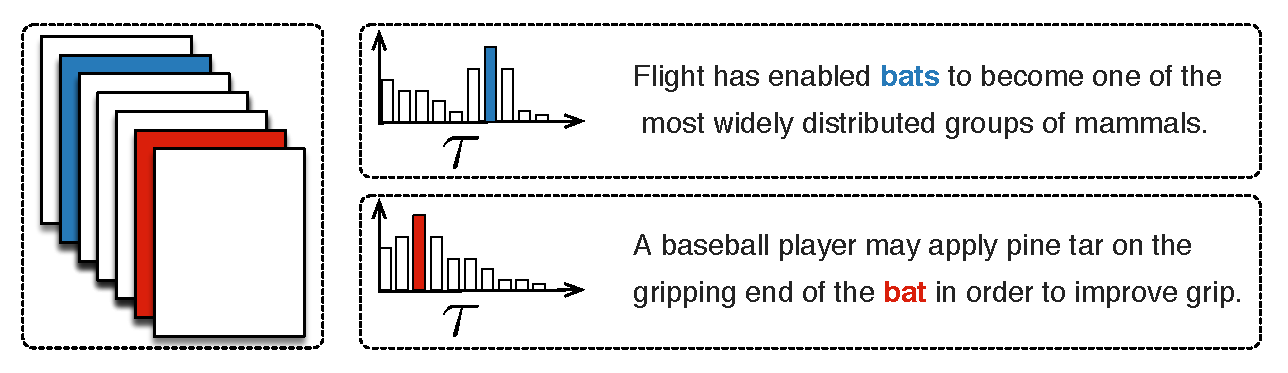
\includegraphics[scale=0.4]{03-research-01/figs/one.pdf} 
  \caption{An example of sentences including the word `bat' from two documents with different topic distribution.}
    \label{modelsfig0}
\end{figure}

Similarly to \citet{neelakantan2014efficient}, we use neighboring words %of a particular target word 
to detect the meaning of the context, however,
we also use the two HDP distributions. 
By doing so, we take advantage of the topic of the document beyond the scope of the neighboring words, which is helpful when the immediate context of the target word is not sufficiently informative. 
We modify the Skipgram model \citep{mikolov2013efficient} to obtain multiple topic-sensitive representations per word type using topic distributions.

Additionally, the context vectors of a word type with multiple topics are shared in our model.
This is especially beneficial for infrequent words, where a rare sense of the word can use the contextual information of other senses of the word.
%In addition, In our models the contexts of the identical target words with different topics are shared which 
%reduces the sparsity problem and provides a better representation estimation for rare words.
%In addition, \citet{neelakantan2014efficient} cluster context windows
%unlike \citet{neelakantan2014efficient}, we train for every sense of a word individually. and do not cluster the context windows
%This %In our models the contexts of the identical target words with different topics are shared which 
%reduces the sparsity problem and provides a better representation estimation for rare words.
We assume that meanings of words can be determined by their contextual information and use the distribution over topics to differentiate between occurrences of a word in different contexts, i.e., documents with different topics (see example in Figure~\ref{modelsfig0}).
We propose three different approaches illustrated in Figures~\ref{modelsfigH} and \ref{modelsfigS}:
two methods with hard topic labeling of words and one with soft labeling.
In the following sections, we discuss each of these model variants in detail.
  
\subsection{Hard topic-labeled representations}
\label{sect:hardReps}

\begin{figure*}[ht!]
\centering
\begin{subfigure}[t]{0.285\textwidth}
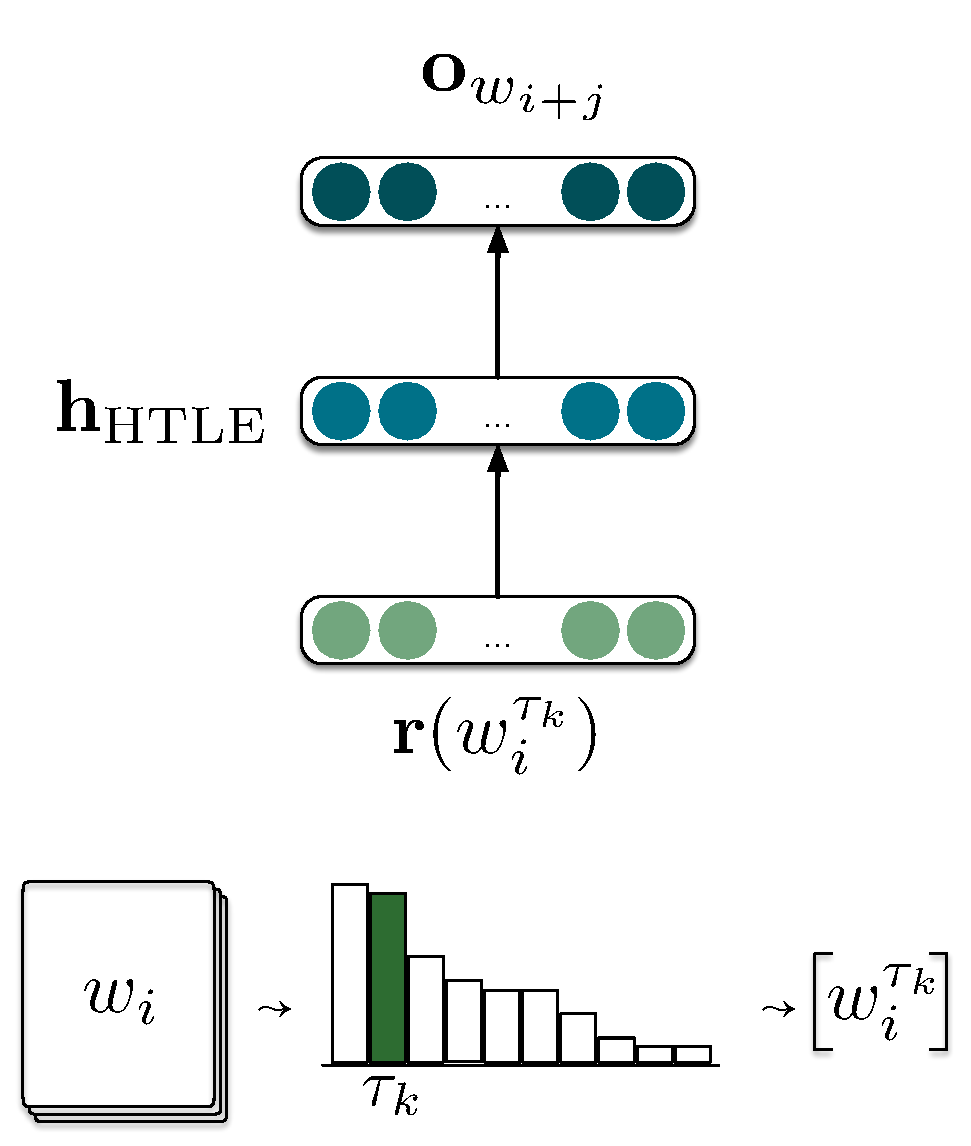
\includegraphics[width=\linewidth]{03-research-01/figs/fig1.pdf}
\caption{\textbf{HTLE}: Hard-topic labeled representations model}
\end{subfigure}
\hspace{0.15\textwidth}
\begin{subfigure}[t]{0.315\textwidth}
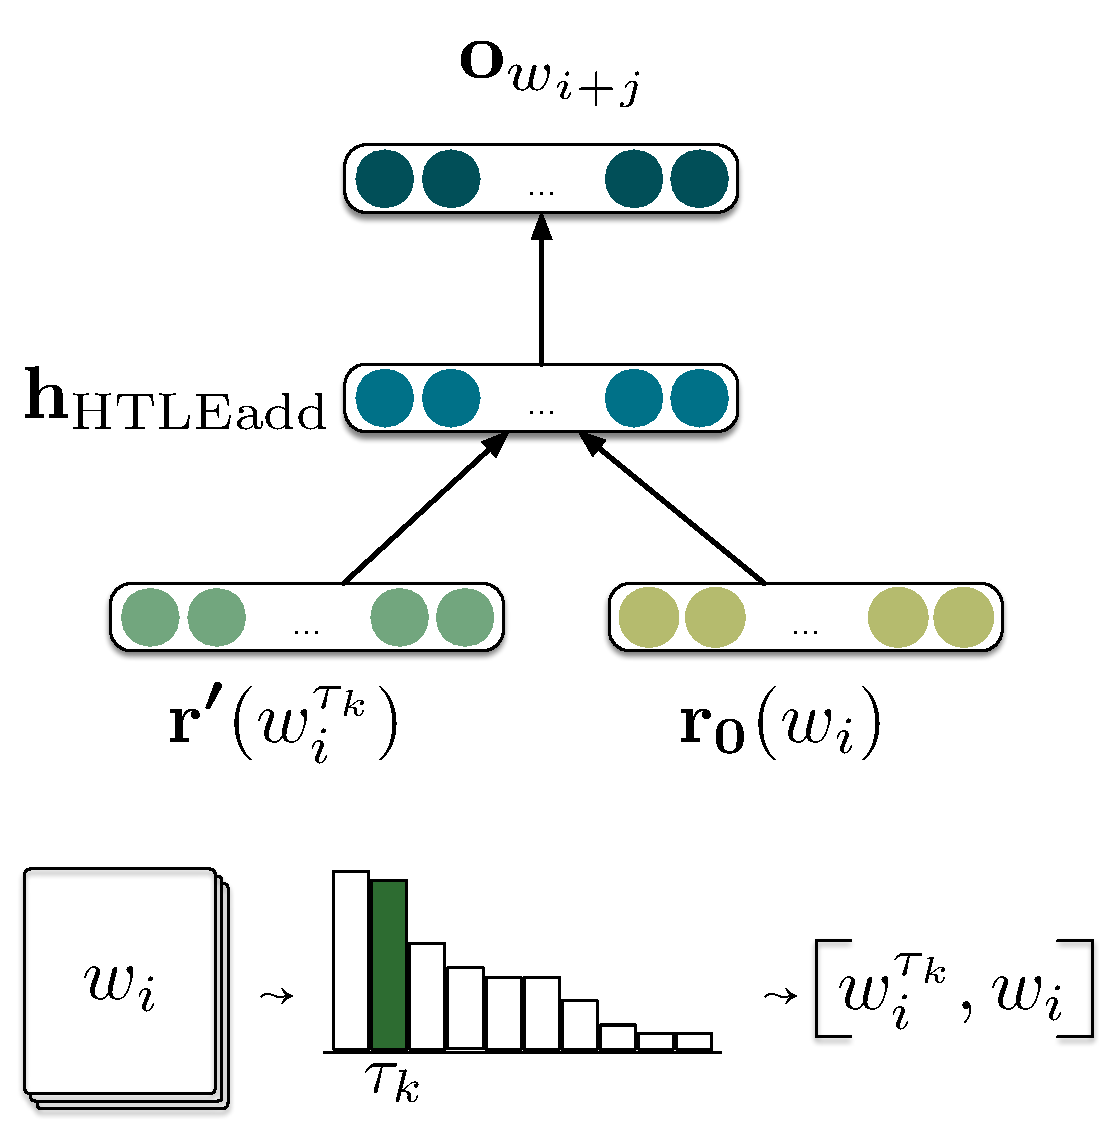
\includegraphics[width=\linewidth]{03-research-01/figs/fig2.pdf}
\caption{\textbf{HTLEadd}: Hard topic-labeled representations plus generic word representations model}
\end{subfigure}
\caption{Illustrations of two proposed models with hard-labeling topics in this chapter. \label{modelsfigH}}
\end{figure*}

In the hard-labeling approach, we assign exactly one topic to each word based on sampling from the topic distribution.
We use the trained HDP model to label every word in the training data with the chosen topic ID.

Our first model variant (Figure~\ref{modelsfigH} (a)) considers each word-topic pair as a separate vocabulary entry.
To reduce sparsity on the context side and share the word-level information between similar contexts, we use topic-sensitive representations for target words (input to the Skipgram network) and standard, i.e., unlabeled, word representations for context words (output to the Skipgram network). Note that this results in different input and output vocabularies.
The training objective is then to maximize the log-likelihood of context words $w_{i+j}$ given the target word-topic pair $w_{i}^{\tau}$:
%
\begin{align}\small
\mathcal{L}_{HardT\textrm{-}SG} = \frac{1}{I} \sum_{i=1}^I \sum_{\substack{-c \le j \le c \\ j \ne 0}}{\log p(w_{i+j} \mid w^{\tau}_{i})}
\end{align}
\noindent%
%
where $I$ is the number of %running 
words in the training corpus, $c$ is the context %window 
size and $\tau$ is the topic assigned to $w_i$ by HDP sampling.
$\vt{o}_{w_{i+j}}$ is the context (i.e., output) representation for the word $w_i$.
Note that $w_i$ is an occurrence of word $w$ in context $[i-c, i+c]$.

The embedding of a word in context $\vt{h}({w_i})$ is obtained by simply extracting the row of the input lookup table (\vt{r}) corresponding to the HDP-labeled word-topic pair:
\begin{equation}\label{eq:HTLE}
\vt{h}_\textrm{HTLE}({w_i}) = \vt{r}(w_i^{\tau})
\end{equation}

A possible shortcoming of the HTLE model is that the representations are trained separately and information is not shared between different topic-sensitive representations of the same word. 
To address this issue, we introduce a model variant that learns multiple topic-sensitive word representations and generic word representations simultaneously (Figure~\ref{modelsfigH} (b)). 
In this variant (HTLEadd), the target word embedding is obtained by adding the word-topic pair representation ($\vt{r'}$) to the generic representation of the corresponding word ($\vt{r_0}$):
\begin{equation}\label{eq:HTLEadd}
\vt{h}_\textrm{HTLEadd}({w_i}) = \vt{r'}(w_i^\tau) + \vt{r_0}(w_i)
\end{equation}

This representation captures both the generic and the contextual meaning of the word.

\begin{figure*}[hbt!]
\centering
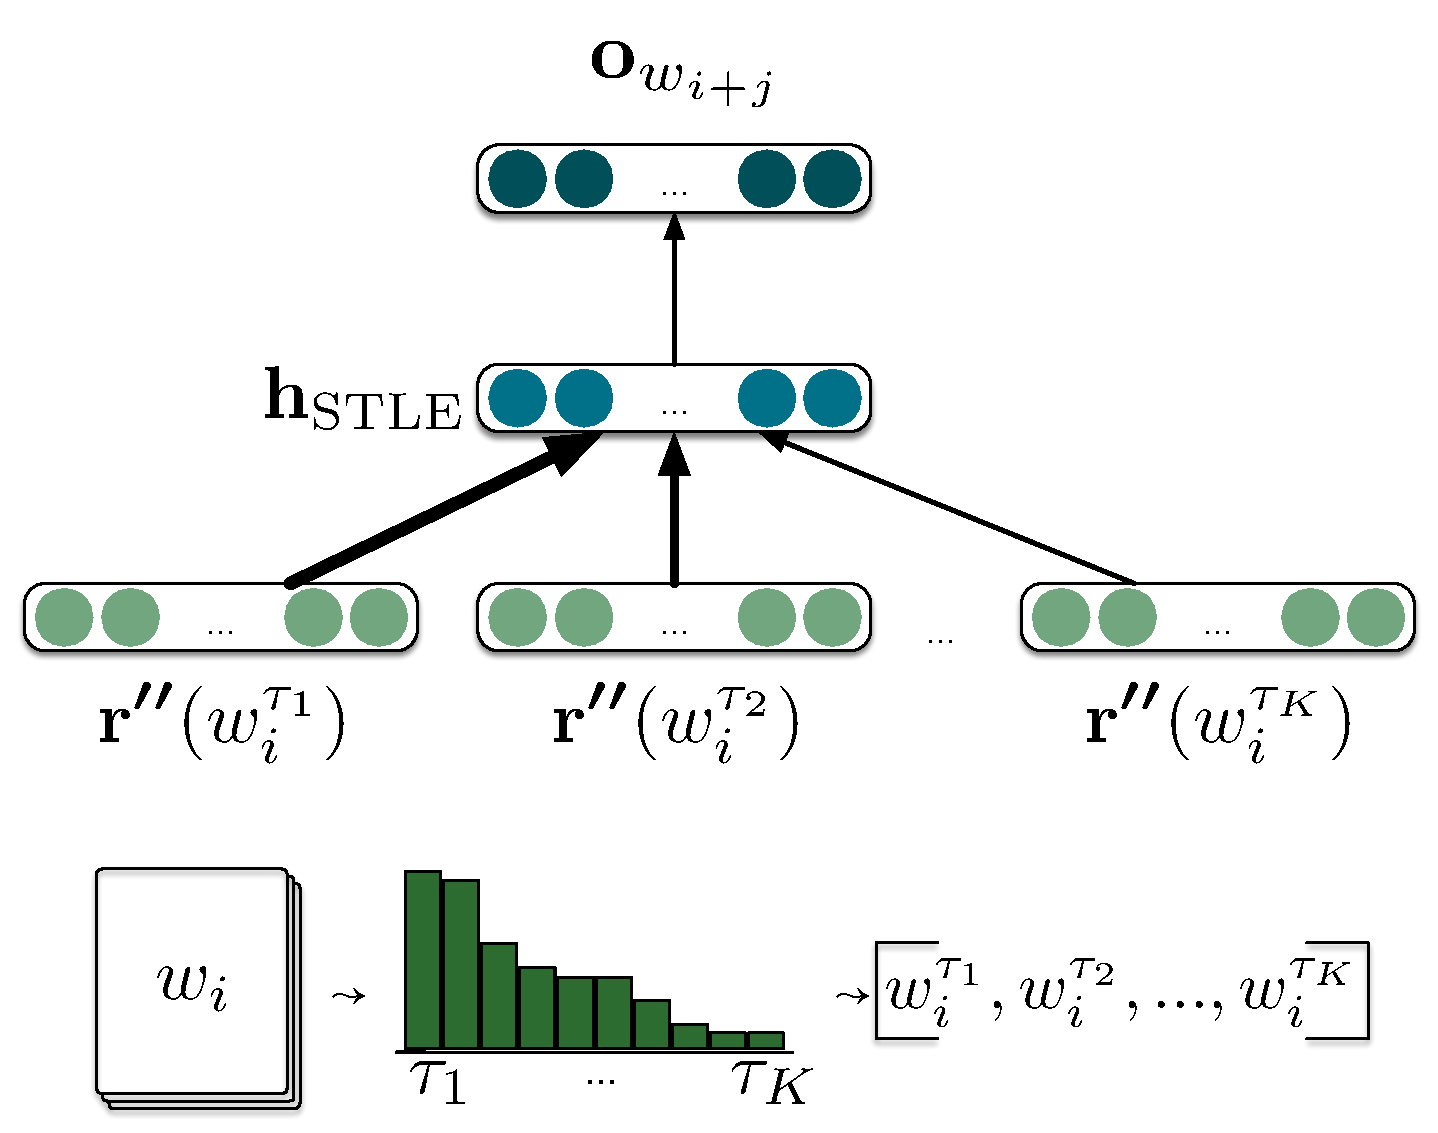
\includegraphics[scale=0.2]{03-research-01/figs/fig3.pdf}
\caption{Illustration of our soft topic-labeled representation model (STLE). \label{modelsfigS}}
\end{figure*}

\subsection{Soft topic-labeled representations}
\label{sect:softReps}

 \begin{table} \setlength{\tabcolsep}{0.2em}
\centering\small
\caption{Nearest neighbors of three examples in different representation spaces using cosine similarity. \textbf{word2vec} and \textbf{GloVe} are pre-trained embeddings from \protect\citep{mikolov2013efficient} and \protect\citep{pennington2014glove}, respectively. \textbf{SGE} is the Skipgram baseline and \textbf{HTLE} is our topic-sensitive Skipgram (cf. Equation~(\ref{eq:HTLE})), both trained on Wikipedia. $\tau_k$ stands for HDP-inferred topic $k$.\label{embs}}
\begin{tabular}{@{\extracolsep{4pt}} c|l|l|l|ll @{}}
\toprule
  \multicolumn{3}{c}{\bf Pre-trained}   & \multicolumn{3}{c}{\bf  Trained on Wikipedia}  \\ \cline{2-3} \cline{4-6} 
& \bf word2vec & \bf Glove & \bf SGE & \bf HTLE: $\tau_1$ & \bf HTLE: $\tau_2$ \\ \toprule
\multirow{10}{*}{\rotatebox[origin=c]{90}{\textbf{bat}}}  &bats&bats&uroderma&ball&vespertilionidae \\
&batting&batting&magnirostrum&pitchout&heran\\
&Pinch\_hitter\_Bray\textellipsis&Bat&sorenseni&batter &hipposideros\\
&batsman&catcher&miniopterus&toss-for&sorenseni\\
&batted&fielder&promops&umpire &luctus\\
&Hawaiian\_hoary&hitter&luctus&batting &coxi\\
&Lelands.com\textellipsis&outfield&micronycteris&bowes &kerivoula\\
&yelled\_Cheater&hitting&hipposideros&straightened &natterer\\
&wicketkeeper\_Andr\textellipsis&batted&chaerephon&fielder &nyctophilus\\
&lefthanded\_batter&catchers&pteronotus&flies &artibeus\\
%&Batting&balls&bats&ball-a&carollia\\
%&skipper\_Nicky\_Boje&slugger&gallagheri&yardley &pteronotus\\
%&batsmen&hitters&saccolaimus&hitting &lucifugus\\
%&baseman\_mitt&Bats&carollia&base &nasutus\\
%&uppercutting&baseball&ball-a&plate &macleayii\\
%&fielder&batsman&emballonura&batsmen &nosed \\
\midrule
\multirow{10}{*}{\rotatebox[origin=c]{90}{\textbf{jaguar}}}  & jaguars&jaguars&electramotive&ford &wiedii \\
&Macho\_B&xk8&vk66de&bmw &	puma \\
&panther&xj6&viper&chevrolet &	margay\\
&lynx&xjs&id66&honda &	tapirus\\
&rhino&panther&xj666&porsche &	jaguarundi\\
&lizard&xkr&roadster&multimatic&	yagouaroundi\\
&tapir&xj8&saleen&monza &	vison\\
&tiger&mercedes&siata&nissan &	concolor\\
&leopard&Jaguar&enetered&xj&	tajacu\\
& Florida\_panther	& porsche	& chevrolet	& dodge &		tayassu \\
\midrule
\multirow{10}{*}{\rotatebox[origin=c]{90}{\textbf{appeal}}}  &appeals&appeals&court&court&sfa  \\
&appealing&appealed&appeals&case&steadfast\\
&appealed&appealing&appealed&appeals&lackadaisical\\
&Appeal&Appeal&carmody&appealed&assertions\\
& rehearing&court&upheld&decision&lack\\
& apeal&decision&verdict&proceedings&symbolize\\
& Appealing&conviction&jaruvan&disapproves&fans\\
& ceasing\_hostilities\textellipsis &plea&affirmed&ruling&attempt\\
& ruling&sought&appealable&upholding&unenthusiastic\\
& Appeals&dismiss&battin&carmody&cancellation \\
\bottomrule                  
\end{tabular}
\end{table}

The model variants above rely on the hard labels resulting from HDP sampling.
As a soft alternative to this, we can directly %incorporate into our Skipgram model 
include the topic distributions estimated by HDP for each document, see Figure~\ref{modelsfigS}. 
Since the topics are not clearly separated, every identified topic of a word can contribute to the learning process proportional to its value.
%
%
Specifically, for each update, we use the topic distribution to compute a weighted sum over the word-topic representations ($\vt{r''}$):
\begin{equation}\label{eq:STLE}
\vt{h}_\textrm{STLE}(w_i) = \sum_{k=1}^{T}  \ p(\tau_k \mid d_i) \ \vt{r''}(w_i^{\tau_k})
\end{equation}
%\noindent% 
where $T$ is the total number of topics, $d_i$ the document containing $w_i$, and $p(\tau_k \mid d_i)$ the probability assigned to topic $\tau_k$ by HDP in document $d_i$.
%
The training objective for this model is:
%
\begin{align}\small
\mathcal{L}_{SoftT\textrm{-}SG} = \frac{1}{I} \sum_{i=1}^I \sum_{\substack{-c \le j \le c \\ j \ne 0}}{\log p(w_{i+j} \mid w_i, \tau)}
\end{align}


\noindent%
where $\tau$ is the topic of document $d_i$ learned by HDP. 
The STLE model has the advantage of directly applying the distribution over topics in the Skipgram model. 
Also, for each instance, we update all topic representations of a given word with non-zero probabilities, which has the potential to reduce the sparsity problem.

\subsection{Embeddings for polysemous words}

The representations obtained from our models are expected to capture the meaning of a word in different topics.
We now examine whether these representations can distinguish between different word senses.
Table~\ref{embs} provides examples of nearest neighbors. 
For comparison, we include our own baseline, i.e., embeddings learned with Skipgram on our corpus, as well as Word2Vec \citep{mikolov2013distributed} 
and GloVe embeddings \citep{pennington2014glove} 
pre-trained on large data.

\begin{table}
\centering
\small
\caption{Statistics of the degree of polysemy in Wordnet and HTLE. \label{wordnetinfo}} %out of 46255 overlap between wn and ours 
\begin{tabularx}{0.65\textwidth}{lcc}
\toprule
& \textbf{Wordnet} & \textbf{HTLE} \\
\midrule
 Degree of polysemy & 2.08 & 4.79 \\
  Single [sense/representation] words &  26,755 & 21,490 \\
\bottomrule
\end{tabularx}
\end{table}

In the first example, the word \textit{bat} has two different meanings: animal or sport device. We can see that the nearest neighbors of the baseline and pre-trained word representations either center around one primary, i.e., most frequent, meaning of the word, or looks like a mixture of different meanings. 
The topic-sensitive representations, on the other hand, correctly distinguish between the two different meanings. A similar pattern is observed for the word \textit{jaguar} and its two meanings: car or animal.
%
The last example, \textit{appeal}, illustrates a case where topic-sensitive embeddings are not clearly detecting different meanings of the word, despite having some correct words in the lists. %(\textit{unenthusiastic}, \textit{fans})
%there are also errors present. 
Here, the meaning \textit{attract} does not seem to be captured by any embedding set. 

These observations suggest that topic-sensitive representations capture different word senses to some extent.
To quantify the degree of polysemy in our embeddings, we compare it to Wordnet \citep{miller1995wordnet}. 
Wordnet is a manually curated lexical database of English that interlinks different senses of the words through conceptual-semantic and lexical relations.
As a result, words that are found near one another in the network are semantically disambiguated. 
Table~\ref{wordnetinfo} shows statistics for Wordnet and our proposed embedding method.
We observe that the \textit{degree of polysemy} of our embeddings is more than double that of Wordnet.
Note that while in our models we do not explicitly specify the desired number of senses per word type, the hyperparameters have an impact on it: $\gamma$ manages the variability of the global sense distribution and $\alpha$ manages the variability of each word type's selection of senses. These hyperparameters are discussed in Section~\ref{embexpsetup}.

Moreover, we observe that not every topic-sensitive word representation corresponds to a distinct and unique sense. 
In our experiments, we see that at times, multiple embeddings capture the same sense of the word.
However, they are also in close proximity in the embedding space and end up being very similar.
To provide a systematic validation of our approach, we now investigate whether topic-sensitive representations can improve tasks where polysemy is a known issue. 


\section{Evaluation} \label{embevaluationsec}

In this section, we present the setup for our experiments and empirically evaluate our approach on the context-aware word similarity and lexical substitution tasks.

\subsection{Experimental setup} \label{embexpsetup}


%We use the English Wikipedia corpus containing 4.8M documents %and 1B tokens 
All word representations are learned on the English Wikipedia corpus containing 4.8M documents (approximately 1 billion tokens).
Preprocessing of the training data includes lowercasing, removing stop words, and removing words occurring less than 100 times.
The topics are learned on a 100K-document subset of this corpus using the HDP implementation of \citet{teh2006hierarchical}.
%
HDP has two hyperparameters, $\gamma$  and $\alpha$, which control the variability of the global topic distribution and each word's choice of topics, respectively. We do not tune these parameters and following the literature, %set these values to 
we put gamma priors $\gammaa(1, 1)$ and $\gammaa(1, 0.1)$ on hyperparameters $\gamma$ and $\alpha$ respectively. These parameters encourage skewed topic distributions which are typically observed in natural languages \citep{Gale1992}. 
%
Once the topics have been learned, we run HDP on the whole corpus to obtain the word-topic labeling (Section~\ref{sect:hardReps}) and the document-level topic distributions (Section~\ref{sect:softReps}).
%
We train each model variant with window size $c=10$ and different embedding sizes (100, 300, 600) with random initialization. 
All model variants in this chapter are trained on the same training data with the same settings, following suggestions by \citet{mikolov2013efficient} and \citet{levy2015improving}. 

\begin{table}[htb!]
\centering
\small
\caption{Word similarity benchmarks for intrinsic evaluation of word representations. \label{wstab}}
\begin{tabular}{lcl}%@{}}
\toprule
\textbf{Data set} & \textbf{Word pairs} & \textbf{Reference} \\
\midrule
RG & 65 & \citet{Rubenstein:1965:CCS:365628.365657} \\ %
%MC & 30 & \citet{miller1991contextual} \\ %
WS353 & 353 &  \citet{Finkelstein:2001:PSC:371920.372094} \\ %
%YP-130 & 130 &  \citet{Yang06verbsimilarity} \\  
MTurk287 & 287 &  \citet{Radinsky:2011:WTC:1963405.1963455} \\ %
%MTurk771 & 771 &  \citet{Halawi:2012:LLW:2339530.2339751} \\
MEN & 3000 &  \citet{bruni-etal-2012-distributional} \\ %
RW & 2034 &  \citet{luong-etal-2013-better} \\ %
%Verb & 144 &  \citet{baker-etal-2014-unsupervised} \\
SimLex & 999 &  \citet{hill-etal-2015-simlex} \\ %
\bottomrule
\end{tabular}
\end{table}

\subsection{Word similarity task}

The most popular intrinsic evaluation of static word representations is the word similarity task. 
In this task, a list of pairs of words with their similarity scores judged by human annotators is provided. 
The goal is to measure how well the word vector representations capture the notion of word similarity by ranking the word pairs according to their similarity scores. 
Table~\ref{wstab} provides a list of benchmarks with the number of word pairs in each data set that we use for evaluation. 

Similar to most previous approaches \citep{Radinsky:2011:WTC:1963405.1963455,hassan2011semantic,yih-qazvinian-2012-measuring}, we use Spearman's $\rho$ (rank correlation coefficient) to assess the monotonic relationship between the model's ranking of word pairs and the gold standard's ranking. 

Our models learn multiple embeddings per word, but these benchmarks do not include any context to help distinguish between the vectors.
Therefore we employ several techniques for selecting and combining the representation vectors:
%
\begin{itemize}
\itemsep0em 
\item \textbf{Max}: computes the pairwise similarity between the nearest topic-sensitive embeddings of the word pair.
\item \textbf{Mean}: computes the pairwise similarity between the means of all topic-sensitive embeddings of each word. 
\item \textbf{wMean}: computes the pairwise similarity between the weighted means of all topic-sensitive embeddings of each word. The weights are defined according to the frequency of each topic.
\end{itemize}


Table~\ref{wstabres} provides the results for the word similarity experiments. 
We observe slight improvements in different settings, but there is no clear indication that one model performs best across all data sets. 
It is also clear that each data set has a different level of difficulty, and because of the differences in quality of the word pairs and the definition of \textit{similarity} for the annotators, they are not analogous. 

\begin{table}[tbh!]  \setlength{\tabcolsep}{0.4em} 
\centering
\small
\caption{Spearman's rank correlation performance on word similarity tasks. All vectors are 100-dimensional. \label{wstabres}}
\begin{tabular} {llccccccc} 
\toprule
\multicolumn{1}{c} {} &
  \multicolumn{1}{c} {} &
  \multicolumn{1}{c} {\textbf{RG}} &
  \multicolumn{1}{c} {\textbf{WS353-rel}} &
  \multicolumn{1}{c} {\textbf{WS353-sim}} &
  \multicolumn{1}{c} {\textbf{MTurk287}} &
  \multicolumn{1}{c} {\textbf{MEN}} &
  \multicolumn{1}{c} {\textbf{RW}} &
  \multicolumn{1}{c} {\textbf{SimLex}} \\
\midrule
  \multicolumn{2}{l}{SGE} & 0.77  & 0.44 & 0.69 & 0.66  & \bf 0.71 & \bf 0.38 & 0.29 \\ \midrule
\multirow{3}{*}{\rotatebox[origin=c]{90}{HTLE}} & Max & 0.68 & 0.20 & 0.46 & 0.42 & 0.51 & 0.15 & 0.20 \\
 & Mean & 0.65 & 0.29 & 0.61 & 0.62 & 0.57 & 0.35 & 0.22 \\
 & wMean & 0.48 & 0.32 & 0.40 & 0.55 & 0.50 & 0.08 & 0.10 \\ \midrule
\multirow{3}{*}{\rotatebox[origin=c]{90}{HTLEadd}}  & Max &\bf  0.81 &  0.30 & 0.57 & 0.56  & 0.63 & 0.24 & 0.22  \\
 & Mean & 0.77 & 0.42 & 0.67 & \bf 0.68 & 0.69 & 0.36 & 0.28 \\
 & wMean & 0.60 & 0.36 & 0.48 & 0.63 & 0.57 & 0.13 & 0.14 \\ \midrule
\multirow{3}{*}{\rotatebox[origin=c]{90}{STLE}}  &Max & 0.74  & 0.43 & 0.69 &0.67 & 0.69 & 0.20 & 0.30 \\
 & Mean & 0.71 & \bf 0.45 & \bf 0.69 & 0.67 &  0.67 & 0.23 & \bf 0.30 \\
 & wMean & 0.65 & 0.43 & 0.64 & 0.65 & 0.68 & 0.16 & 0.24 \\
\bottomrule
\end{tabular}
\end{table}

One of the main concerns of using these benchmarks, in general, is that the notion of word similarity is subjective and there is no clear division between similarity and relatedness \citep{faruqui2016problems,torabi-asr-etal-2018-querying}.
As a result, some data sets penalize representation models that consider two related words as `not similar', while others do not.
For instance, in MEN \citep{bruni-etal-2012-distributional}, the guidelines did not distinguish between similarity and relatedness and gave examples of both similarity (e.g., \textit{"car-automobile"}), and relatedness (e.g., \textit{"wheels-car"}) as valid options to the annotators. 
The instructions for the SimLex data set \citep{hill-etal-2015-simlex}, however, included guidelines for the annotators with examples of related pairs (e.g., \textit{"car-tyre"}) that are \textit{not} to be labeled similar.

\citet{faruqui2016problems} evaluated several issues of the word similarity task.
These include low correlation with extrinsic evaluation, no consideration of polysemy, absence of statistical significance, and semantic versus task-specific embeddings. 
To specifically address the lack of context to identify polysemous words, \citet{huang2012improving} proposed the Stanford contextual word similarity data set (SCWS). In the following subsection, we evaluate our embeddings using this data set. 
 

\subsection{Context-Aware word similarity task}

As mentioned before, there are multiple test sets available for intrinsic evaluation of embeddings, but in almost all of them word pairs are considered out of context. 
To evaluate our static embeddings intrinsically, we use the SCWS data set \citep{huang2012improving}. 
To the best of our knowledge, this was the only word similarity data set considering word context at the time our models were developed.
Note that more recently, instead of intrinsic evaluations, the performance of dynamic contextual embeddings is typically evaluated on downstream NLP tasks \citep{peters-etal-2018-deep,devlin-etal-2019-bert}. 

The SCWS data set contains word pairs and their respective contexts with average human ratings indicating the similarity of the target words.
Table~\ref{iwdtexample} presents examples of word pairs and their contexts in SCWS. 
\begin{table}[tbh!]
\caption{Examples from SCWS data set. Each example includes the word pair (identical or non-identical), their corresponding contexts, and the average human score between 0 and 10 to indicate the similarity. \label{iwdtexample}} %Subscripts are the topic IDs assigned to the word in the given context.   
\centering
\small
\renewcommand{\tabcolsep}{3pt}
\begin{tabularx}{\textwidth}{lX}
\toprule
\textbf{Word pair} & \textit{bitter,  bitter}  \\
  \hdashline
$\text{context}_1$ & It has an aromatic, warm and slightly \underline{bitter} taste. \\
$\text{context}_2$ & AK - a very common beer name in the 1800s - was often referred to as a "mild \underline{bitter} beer" interpreting "mild" as "unaged". \\
  \hdashline
Human score & 6.0 \\
\midrule
\textbf{Word pair} & \textit{ bitter,   resentful}       \\
  \hdashline
$\text{context}_1$ &  Named for the tattoos they decorated themselves with and \underline{bitter} enemies of encroaching Roman legions, the Picts fired Howard's imagination and crystallized in him a love for barbarians and outsiders from civilization who lived lives of great hardship and struggle but also great freedom and verve. \\
$\text{context}_2$ &   Legge-Bourke had been hired by Prince Charles as a young companion for his sons while they were in his care, and Diana was extremely \underline{resentful} of Legge-Bourke and her relationship with the young princes.\\
  \hdashline
Human score & 9.0 \\
\midrule
\textbf{Word pair} & \textit{bitter,     taste}  \\
  \hdashline
$\text{context}_1$ & This practice began during the Prohibition as a means of covering the \underline{bitter} taste. \\
$\text{context}_2$ & Once it has decayed, it leaves no \underline{taste} or odor in drinking water. \\
  \hdashline
 Human score  & 7.0 \\
  %\midrule
%\textbf{Word pair} & \textit{bitter, ale}  \\
  %\hdashline
%$\text{context}_1$ &  The designation of such beers as "\underline{bitter}" or "mild" has tended to change with fashion. \\
%$\text{context}_2$ &  When the beer has fermented, it is packaged either into casks for cask \underline{ale} or kegs, aluminium cans, or bottles for other sorts of beer. \\
  %\hdashline
% Human score & 8.0 \\
 \bottomrule
\end{tabularx}
\end{table}
To evaluate our models on SCWS, we run HDP on the data treating each word's context as a separate document.
We compute the similarity of each word pair as follows:
\begin{align}\small
\text{Sim}(w_1, w_2) &= \cos(\vt{h}(w_1), \vt{h}(w_2)) 
\end{align}
where $\vt{h}(w_i)$ refers to any of the topic-sensitive representations defined in Section~\ref{sect:model}. 
Note that $w_1$ and $w_2$ can refer to the same word.

%%%%%%%%%%
We compare our models to various baselines: The Skipgram model (SGE), the context-aware Skipgram model (SGE + context), and the best-performing multi-sense embeddings model per word type (MSSG) \citep{neelakantan2014efficient}. 
The context-aware Skipgram baseline (SGE + context) computes the average pairwise cosine similarity between a target word in each context with every word in the opposing context.  

For MSSG we use the best performing similarity measure (avgSimC) as proposed by \citet{neelakantan2014efficient}:
%
\begin{align}\small \label{mssgavgsim}
\text{avgSimC}(w_1, w_2)  = \sum_{j=1}^{K} \sum_{i=1}^{K} P(w_1, c_1, i)P(w_2, c_2, j) d(\vt{v}(w_1, i), \vt{v}(w_2, j))
\end{align}

\noindent where $P(w, c, k)$ is the probability that $w$ takes the $k$-th sense given context $c$.
$\vt{v}(w, k)$ is the embedding for word $w$ with assigned sense $k$.
$d(\vt{v}(w_1, i'), \vt{v}(w_2, j'))$ is the similarity measure between the given embeddings $\vt{v}(w_1, i')$ and $\vt{v}(w_2, j')$.
avgSimC measures the similarity between each pair of senses by how well each sense fits the context at hand.
%%%%%%%%%%

Table~\ref{scws} provides the Spearman's correlation scores for different models against the human ranking. 
We see that with dimensions 100 and 300, two of our proposed models obtain slight improvements over the baseline. 
However, for higher dimensions (embedding size 600), the MSSG model is the best performing system. 

\begin{table}[tbh!]
\centering
\small
\caption{Spearman's rank correlation performance for the Word Similarity task on SCWS \citep{huang2012improving}.\label{scws}}
\begin{tabular}{lccc}%@{}}
\toprule
                            & \multicolumn{3}{c}{\textbf{Dimension}} \\ \cmidrule(r){2-4}
      \textbf{Model}        & 100         & 300         & 600         \\ \midrule
SGE + context  \citep{mikolov2013efficient}  &     0.59        &    0.59         &      0.62       \\
MSSG \citep{neelakantan2014efficient} & 0.60 & \bf 0.61  & \textbf{0.64} \\\cmidrule(r){1-4}
HTLE          &     \textbf{0.63}        &       0.56      &       0.55      \\
HTLEadd              &         0.61    &      \textbf{0.61}       &      0.58       \\
STLE                      &     0.59        &      0.58       &       0.55      \\ \bottomrule
\end{tabular}
\end{table}

The main advantage of having multiple embeddings per word for different meanings is in comparing pairs of identical word with ambiguous meanings. 
With multiple representations per word, we can have a better estimation of similarities for identical words, given that we detect different senses correctly. 
 %
Spearman's rank correlation between the two systems is based on the average differences between the two ranks of each observation. 
To further understand the performance of our models, we look into the rank differences for the two types of word pairs in SCWS (identical and non-identical) and the two types of embeddings (assigning the same topic or not).
The former explicitly evaluates the performance of our models on identical words, and the latter evaluates the impact of the topic-labeling step.
This results in four categories for comparison.
%: identical words and non-identical words with the same topic assignment or not.

   \begin{figure}[htb!]
\centering
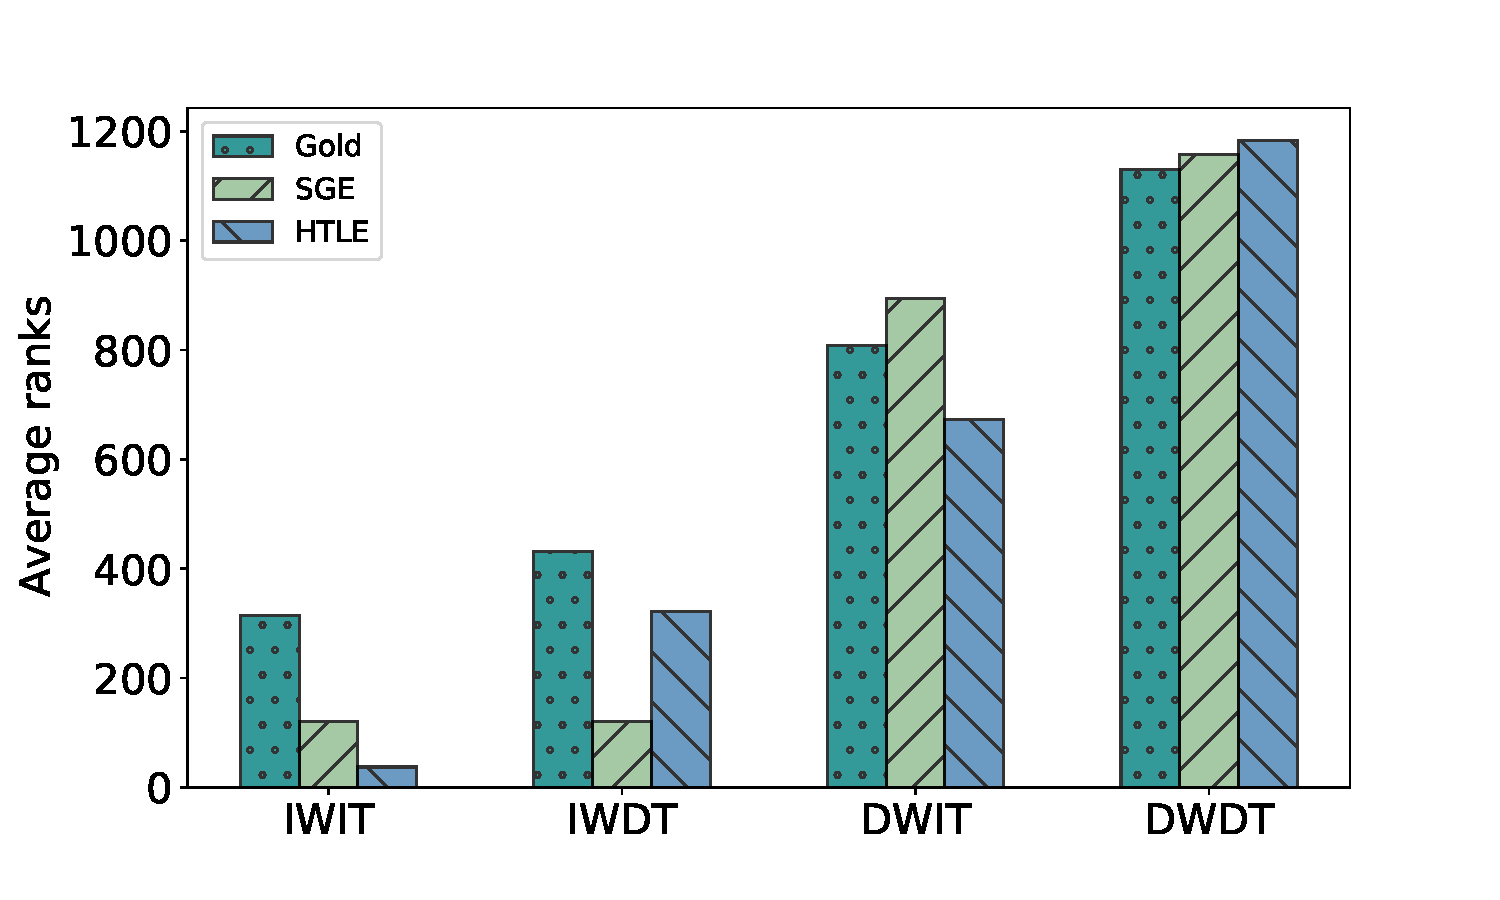
\includegraphics[scale=0.4]{03-research-01/figs/iwits2.pdf} 
  \captionof{figure}{Average absolute rank of the baseline embeddings and the HTLE embeddings in four categories, where being closer to the gold rankings is better. The categories are marked with a combination of these labels:
  %Average ranks of different embedding spaces in four categories of word and topic. 
  \textbf{I}: identical, \textbf{D}: different. \textbf{W}: word, \textbf{T}: topic. %Lower values are better.
  For instance \texttt{IWDT} is the category of word pairs where \textit{\textbf{i}dentical \textbf{w}ords have \textbf{d}ifferent \textbf{t}opics}. Examples of the categories are presented in Table~\ref{iwdtexample}.}
  \label{scwsbar}
   \end{figure}
   
Since the difficulty of each category is different, we expect different performances from the models.
Figure~\ref{scwsbar} shows the average absolute rank of the baseline embeddings and the HTLE embeddings with 300 dimensions in these four categories. 
The gold rank, which is the ranking of all word pairs in the data set according to human judgments, is also shown for each category.
The best-performing model is the one that is the closest to the gold ranking.
Note that the gold rank naturally increases when words are different in comparison to when they are the same. 
%This displays the distribution of the test data where the number of identical words that are also semantically similar is higher. 
   
One can see that for identical words, labeled with different topics, \texttt{IWDT}, the rank assigned by topic-sensitive embeddings is much closer to the gold ranking than the one produced by the baseline. 
The average rank is also still higher when considering both categories of identical words: \texttt{IWDT} and \texttt{IWIT}.
This indicates that the estimation of the similarity scores of identical words is notably more accurate in our model. 
%
However, for non-identical word pairs (\texttt{DWIT} and \texttt{DWDT}), the rank difference is higher for topic-sensitive embeddings and since the evaluation set consists of mostly non-identical word pairs, the correlation with gold ranking decreases in total in comparison with baseline word embeddings. 

\subsection{Lexical substitution task}

Continuing our evaluation of word representations, in this section, we explore the lexical substitution task. 
This task requires one to identify the best replacements for a word in a sentential context. The replacements should be both semantically compatible with the word, and syntactically correct in the context. For example:

\vspace{1mm}

\begin{center}\small
\setlength{\tabcolsep}{20pt}
\begin{tabular}{l l}
\textbf{sentence} & \textbf{substitutions} \\ \hline
The sun was \underline{bright}. & \textit{luminous, colorful}  \\
He was \underline{bright} and independent.  & \textit{intelligent, clever, smart} \\
\end{tabular}
\end{center}

\vspace{1mm}

The presence of many polysemous target words makes this task more suitable for evaluating sense embeddings. %Instead of using an open vocabulary, 
Following \citet{melamud2015simple}, we pool substitution candidates 
from different instances and rank them by the number of annotators that selected them for a given context. 
We use two evaluation sets: LS-SE07 \citep{mccarthy2007semeval}, and LS-CIC \citep{kremer2014substitutes}.
The Concept-in-Context (LS-CIC) set for the lexical substitution task is a large-scale corpus constructed by crowdsourcing \citep{kremer2014substitutes} and contains a more extensive set of words. 
The main difference between LS-CIC and LS-SE07 is that the former was constructed as a large-scale "all-words" corpus, while LS-SE07 mostly includes ambiguous words. 

Unlike previous work \citep{DBLP:conf/emnlp/SzarvasBH13,kremer2014substitutes,melamud2015simple}, we do not use any syntactic information in our models, % during training or testing, 
motivated by the fact that high-quality parsers are not available for most languages.
% The main reason is that for most languages parsers are not available, hence we only focus on discovering semantic relations. 
The evaluation is performed by computing the Generalized Average Precision (GAP) score \citep{kishida2005property}. %Below we discuss the evaluation pipeline and analyze the performance of the models. 
Given a gold standard of size $R$ of ranked candidates, the GAP score is defined as:
\begin{equation}
\small
\textrm{GAP} = \frac{\sum_{i=1}^n I(x_i) p_i}{R'}    \quad \quad \quad         R' = \sum_{i=1}^R I(y_i)\overline{y}_i
 \end{equation}
 
\noindent where $x_i$ is a binary variable symbolizing whether the $i$-th candidate as ranked by the model is in the gold standard and $n$ is the number of candidates to be ranked. 
$I(x_i)$ is one if $x_i$ is larger than zero, and otherwise, it is zero. 
$\overline{y}_i$ is the average weight of the ideal ranked list in the gold standard.


In order to rank substitution candidates, we compute the similarity between the target word and each candidate similar to \citet{melamud2015simple} but adapt it to include topic distributions as well as context words for word embeddings. 
%As for the word similarity task, 
We run HDP on the evaluation set % differently from the SCWS task, we cannot have topic information 
and compute the similarity between target word $w_t$ and each substitution $w_s$ using two different inference methods in line with how we incorporate topics during training.
We define the first method, Sampled \textit{(Smp)}, as:
\begin{equation}
\small
\cos(\vt{h}(w_s^\tau), \vt{h}(w_t^{\tau'})) +  \frac{\sum_{c}  \cos(\vt{h}(w_s^{\tau}), \vt{o}(w_c)) }{C},  
 \end{equation}
 
\noindent 
and define the second method, Expected \textit{(Exp)}, as:
\begin{equation}
\small
\begin{split}
\sum_{\tau, \tau'}  \ p(\tau) \ p(\tau') \cos(\vt{h}(w_s^\tau), \vt{h}(w_t^{\tau'})) +  \frac{\sum_{\tau,c}  \cos(\vt{h}(w_s^{\tau}), \vt{o}(w_c)) \ p(\tau) }{C},  
\end{split}
\end{equation}

\noindent where $p(\tau)$ and $p(\tau')$ are the topic probabilities, $\vt{h}(w_s^\tau)$ and $\vt{h}(w_t^{\tau'})$ are the representations for substitution word $s$ with topic $\tau$ and target word $t$ with topic $\tau'$ respectively (see Section~\ref{sect:model}),
$w_c$ are context words of $w_t$ taken from a sliding window of the same size as the embeddings,
$\vt{o}(w_c)$ is the context (i.e., output) representation of $w_c$, and $C$ is the total number of context words.
Note that these two methods are consistent with how we train HTLE and STLE.
%
\begin{table}[bht!]
\centering
\small
\setlength{\tabcolsep}{8pt}
\caption{\label{embs_tables00}GAP scores on LS-SE07 and LS-CIC sets. For \textsc{SGE + context} we use the \textit{context} embeddings to disambiguate the substitutions. Improvements over the best baseline (MSSG) are marked $^\blacktriangle$ at $p<.01$ and $^\vartriangle$ at $p < .05$.} 
\begin{tabular}{@{\extracolsep{4pt}}lcllllll@{}}
\toprule
                           && \multicolumn{3}{c}{\textbf{LS-SE07}}  & \multicolumn{3}{c}{\textbf{LS-CIC}} \\ 
                           \midrule
                                                      && \multicolumn{3}{c}{Dimension} &  \multicolumn{3}{c}{Dimension}   \\ 
                                                      \cmidrule{3-5}  \cmidrule{6-8}
              \textbf{Model}      & \textbf{Infer.}       & 100         & 300         & 600       & 100         & 300         & 600     \\ \midrule
SGE  &   \multirow{3}{*}{n/a}  & 36.2          &      40.5       &      41.1   &      30.4     &       32.1      &       32.3       \\
SGE + context  &  &      36.6       &       40.9      &     41.6   &  32.8      &    36.1         &      36.8         \\
MSSG & & 37.8 & 41.1 & 42.9 & 33.9 & 37.8 &  39.1 \\
\midrule
HTLE    & \multirow{3}{*}{Smp} & 39.8$^\blacktriangle$   & 42.5$^\blacktriangle$  &   43.0$^\blacktriangle$  & 32.1 & 32.7 &  33.0   \\
HTLEadd  &   & 39.4$^\vartriangle$   & 41.3$^\blacktriangle$  &   41.8  & 30.4 & 31.5 &    31.7   \\
STLE     &   & 35.2  & 36.7 & 39.0    & 32.9 & 32.3 &  33.9  \\ 
\midrule
HTLE      &  \multirow{3}{*}{Exp}   &     \textbf{40.3}$^\blacktriangle$       &      \textbf{42.8}$^\blacktriangle$       &      \textbf{43.4}$^\blacktriangle$     &     36.6$^\blacktriangle$       &      \textbf{40.9}$^\blacktriangle$        &      \textbf{41.3}$^\blacktriangle$      \\
HTLEadd  &                &       39.9$^\blacktriangle$     &       41.8$^\blacktriangle$       &      42.2       &        35.5$^\vartriangle$     &  37.9$^\vartriangle$          &      38.6      \\
STLE           &     &       38.7$^\vartriangle$      &     41.0         &      41.0       &      \textbf{36.8}$^\blacktriangle$      &  36.8   &     37.1      \\ \bottomrule
\end{tabular}
\end{table}
%
%
The \textit{Smp} method, similar to HTLE, uses the HDP model to assign topics to word occurrences during testing. The \textit{Exp} method, similar to STLE, uses the HDP model to learn the probability distribution of topics of the context sentence and uses the entire distribution to compute the similarity. 
Both of these inference methods can be used with either model.

\medskip

For the context-aware Skipgram baseline (SGE + context), we compute the similarity as follows:
\begin{align}
\similarity(w_s, w_t) = \cos(\vt{h}(w_s), \vt{h}(w_t)) +\frac{\sum_{c} \cos(\vt{h}(w_s), \vt{o}(w_c))}{C} 
\end{align}
This computation uses the similarity between the candidate word and all words in the context, as well as the similarity between target and candidate words.
We also report results for the baseline Skipgram model (SGE) without using the provided context as well as the MSSG model. 
The MSSG baseline uses the best performing similarity measure (Equation~\ref{mssgavgsim}) as proposed by \citet{neelakantan2014efficient} for a context-aware comparison.

Table~\ref{embs_tables00} shows the GAP scores of our models and the baselines. We use the nonparametric rank-based Mann-Whitney-Wilcoxon test 
\citep{sprent2016applied} to check for statistically significant differences between runs. % to check for statistically significant differences } 
We observe that all models using multiple embeddings per word perform better than SGE. 
Our proposed models outperform both SGE and MSSG in both evaluation sets, with more pronounced improvements in the LS-CIC data set. 
Note that we do not require any syntactic information and only focus on the semantic aspect of the task. 
We further observe that our \textit{Exp} method is more robust and performs better for all embedding sizes.  
Moreover, we can see a decrease in GAP for the model variant HTLEadd compared to HTLE. By including a generic representation for each word, different topic representations drift close to each other and obtain a more general meaning of the word as well as the topic-specific meaning. Such representations are not beneficial for this task. %which requires distinguishing between different meanings of a word.


Table~\ref{nvaa} shows the GAP scores broken down by the main word classes: noun, verb, adjective, and adverb. With 100 dimensions, our best model (HTLE) yields improvements across all POS tags, with the largest improvements for adverbs and smallest improvements for adjectives. 
\bgroup
\def\arraystretch{1.25}
\begin{table}[htb!]
\centering
\small
\setlength{\tabcolsep}{.6em}
\caption{GAP scores on the candidate ranking task on LS-SE07 for different part-of-speech categories. \label{nvaa}}
\begin{tabular}{c|l|cccc}
\toprule
& \textbf{Model} &  \textbf{Noun}             & \textbf{Verb}           & \textbf{Adjective}       &  \textbf{Adverb}    \\ % & All  \\ 
\midrule
\multirow{4}{*}{\rotatebox[origin=c]{90}{Dim=100}}  & SGE &  33.1            & 29.2            & 31.7            & 38.2 \\
 & SGE + context   &  37.2            & 31.6            & 37.1            & 42.2           \\
& HTLE &  \textbf{42.4} & \textbf{33.9} & \textbf{38.1} & \textbf{49.7}  \\ 
& STLE & 42.0 & 33.1 & 38.1 & 47.2 \\
\midrule 
\multirow{4}{*}{\rotatebox[origin=c]{90}{Dim=300}}  & SGE & 39.0 & 33.8 & 36.4 & 50.1 \\
 & SGE + context   &  39.2            & 35.0 & 39.0            & \textbf{55.4}   \\
& HTLE &  \textbf{44.9} & \textbf{37.0} & \textbf{41.0} & 50.9      \\ 
& STLE & 42.7 & 37.0 & 39.9 & 50.2 \\
\midrule
\multirow{4}{*}{\rotatebox[origin=c]{90}{Dim=600}}  & SGE & 39.1 & 34.3 & 36.9 & 52.8 \\
 & SGE + context   &   39.7            & 35.7            & 39.9            & \textbf{56.2}\\
& HTLE &  \textbf{45.2} & \textbf{37.2} & \textbf{42.1} & 51.9          \\ 
& STLE & 44.0 & 37.1 & 41.5 &  51.0 \\
\bottomrule
\end{tabular}
\end{table} 
\egroup

When increasing the dimension size of embeddings, the improvements hold up for all POS tags apart from adverbs. It can be inferred that larger dimension sizes capture semantic similarities for adverbs and context words better than other parts-of-speech categories. 
Additionally, we observe for both evaluation sets that the improvements are preserved when increasing the embedding size. 
It should also be noted that the distribution of POS tags in the test set is approximately uniform except for adverbs of which there are fewer instances.

\begin{table}  \setlength{\tabcolsep}{0.5em}
\begin{center}
\small
\caption{\label{lsexample} Examples of word substitution rankings and respective GAP scores. The gold rank includes substitution words and annotators' votes. The models are word embeddings with context (SGE), MSSG \citep{neelakantan2014efficient}, and our topic-sensitive model (HTLE). Target words in the contexts and correct words in the rankings are bold.}
\begin{tabularx}{\textwidth}{lXr}
\toprule
& \textbf{Substitution instance} & \textbf{GAP} \\
\midrule
   \textbf{ (a)}  & {During the siege, George Robertson had appointed Shuja-ul-Mulk, who was a \textit{\textbf{bright}} boy only 12 years old and the youngest surviving son of Aman-ul-Mulk , as the ruler of chitral.} &   \\
 \hdashline
\rule{0pt}{2.5ex} 
   Gold & intelligent (3), clever (3), smart (1) & \\
 \hdashline
\rule{0pt}{2.5ex} 
   SGE   & \textit{shining, luminous, vibrant, brilliant, vivid, colourful, gleam, light, sharp, \textbf{smart},} \ldots & 12.02 \\ % \multirow{3}{*}{\rotatebox[origin=c]{90}{ranks}}  
  MSSG  & \textit{vivid, shining, luminous, brilliant, colourful, vibrant, gleam, sharp, light, talented,} \ldots & 10.34 \\
   HTLE   & \textit{brilliant, gifted, talented, capable, sharp, \textbf{intelligent}, clear, vivid, colourful, shining,} \ldots & 16.00 \\ 
 \midrule
    \textbf{(b.1)}  & Trees on Anmyeondo used to be thick and lush to the extent of prompting a saying, ``you can become \textit{\textbf{rich}} with an axe'', but now only few trees are left due to reckless deforestation since the time of Korea's liberation from Japanese colonial rule.  &  \\
  \hdashline
\rule{0pt}{2.5ex} 
   Gold   & wealthy (5) &  \\
  \hdashline
\rule{0pt}{2.5ex} 
   SGE   & \textit{\textbf{wealthy}, abundant, vibrant, lush, abounding, lavish, ample, valuable,} \ldots & 100 \\
   MSSG  &\textit{ lush, abundant, \textbf{wealthy}, vibrant, abounding, valuable, lavish, ample,} \ldots & 33.33 \\
   HTLE   & \textit{abundant, valuable, lush, abounding, vibrant, ample, high, significant,} \ldots & 7.69 \\ 
 \midrule
\textbf{ (b.2)}  &Africas central problems in the WTO revolve around the imbalances and biases created by \textit{\textbf{rich}} countries in the Uruguay round agreement (URA) . &  \\
 \hdashline
\rule{0pt}{2.5ex} 
   Gold   & wealthy (5) &  \\
  \hdashline
\rule{0pt}{2.5ex} 
   SGE   & \textit{abundant, lush, \textbf{wealthy}, abounding, vibrant, valuable, ample, lavish,} \ldots &  33.33\\
   MSSG  & \textit{abundant, \textbf{wealthy}, vibrant, lush, abounding, lavish, ample, valuable,} \ldots & 50 \\
   HTLE   & \textit{\textbf{wealthy}, abundant, valuable, vibrant, significant, abounding, ample,} \ldots  & 100 \\ 
 \midrule
\textbf{ (c)}   & I feel I can get a lot more done as a selectman by being innovative and \textit{\textbf{fixing}} the problems we have with cash flows, because they occur every year. &  \\
  \hdashline
\rule{0pt}{2.5ex} 
   Gold   & resolve (2), solve (1), mend (1), repair (1) &  \\
  \hdashline
\rule{0pt}{2.5ex} 
   SGE  & \textit{\textbf{resolve}, \textbf{mend}, \textbf{repair}, heal, cure, improve, correct, stick, do, patch,} \ldots  &  79.45  \\
    MSSG  & \textit{do, \textbf{mend}, heal, cure, \textbf{resolve}, \textbf{repair}, correct, improve, stick, patch,} \ldots & 29.04 \\
   HTLE   & \textit{do, improve, heal, \textbf{repair}, cure, \textbf{resolve}, \textbf{mend}, determine, stick,} \ldots   & 21.72  \\ 
 \bottomrule
\end{tabularx}
\end{center}
\end{table}

Our findings confirm \citet{li-jurafsky:2015:EMNLP}'s observations to some extent: 
Higher dimension embeddings capture part of the information on semantic relations that models with multiple embeddings per word capture.
In our experiments, SGE with 600 dimensions performs better than HTLE with 100 dimensions. 
Given a relevant semantic task, this advantage of having multiple embeddings per word can be observed more appropriately regardless of dimension.
   
\section{Qualitative analysis} \label{embindepth}

In this section, we discuss some properties of our representations and provide an analysis of the semantic information captured by topic-sensitive embeddings in the lexical substitution evaluation. 
Table~\ref{lsexample} illustrates the performance of different models by providing examples from the lexical substitution task LS-SE07. 
In Table~\ref{lsexample} (a), for the word \textit{`bright'}, we observe that our model captures the meaning of the word in the context \textit{(`talented')} and provides a sensible substitution ranking, but the GAP scores are low. 
This is due to the gold substitution list being incomplete and the highest-ranking words of our model, despite matching the context, are not in the gold ranking. SGE and MSSG however, rank the candidates belonging to a different sense (\textit{`shiny'}) higher. 


   
    \begin{figure}   
\centering
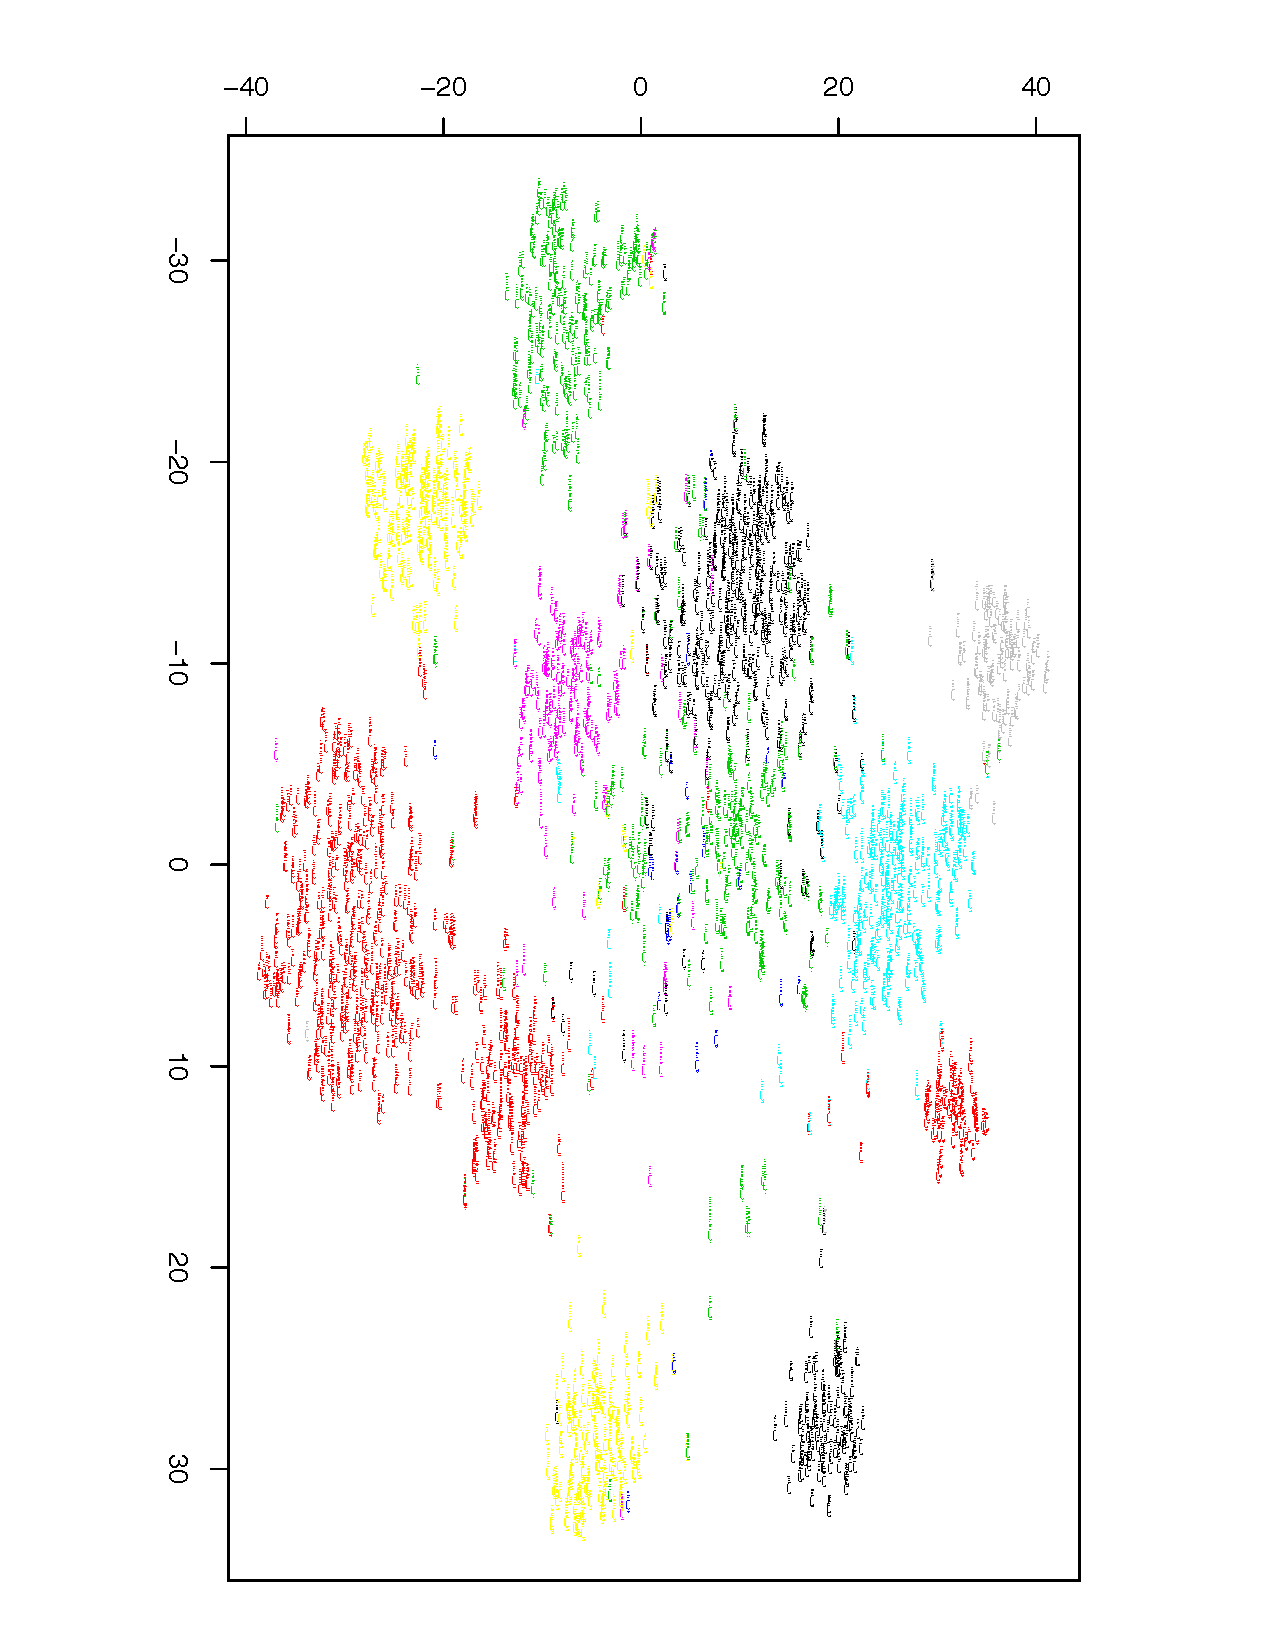
\includegraphics[scale=0.7]{03-research-01/figs/vecvis-rotated.pdf} 
  \captionof{figure}{Visualizing a subset of word-topic pairs using t-SNE to showcase topic assignment separations. Colors distinguish topics. We observe that words that are labeled the same topics end up in the same clusters. }
  \label{vecvis}
   \end{figure}
   
Additionally, Table~\ref{lsexample} provides an example of two different contexts for the same word \textit{`rich'}. In Table~\ref{lsexample} (b.1), the topic of the sentence for the word \textit{`rich'} was learned correctly, but it is misleading for the substitution because the meaning of the word changes in the local context and SGE and MSSG perform better than our model and rank the correct substitution \textit{`wealthy'} higher. 
However, for the same word (\textit{`rich'}) in a different context, Table~\ref{lsexample} (b.2), the topic-sensitive model obtains a more accurate substitution ranking and SGE fails to identify the meaning of the word (\textit{`wealthy'}) in the context.
Example (c) in Table~\ref{lsexample} provides an instance for substituting the word \textit{`fixing'} in which we achieve a higher GAP score by using SGE. Here, both MSSG and our model detect an inaccurate sense for the context (\textit{`heal'}) and rank the words accordingly. 

These examples show that when we learn multiple embeddings per word, we can disambiguate words in context to a greater degree. 
Comparing the MSSG and the HTLE model, we see a slight difference in results.
One distinction between the MSSG model and the HTLE model is their definition of context.
The former uses a context window of length 10 \citep{neelakantan2014efficient} and the latter uses a context window of length 10 as well as the document-level (in this case the complete sentence) topical information. 
While both models perform similarly, HTLE can be more effective when requiring larger contexts for disambiguation.

Figure~\ref{vecvis} uses t-SNE \citep{7b54165e73a3424b8820136bcf61ca89} to visualize the embeddings of a subset of word-topic pairs in the vocabulary with colors distinguishing between topics. 
This figure gives us a basic understanding of the vector space and the distribution of topics.
We observe that in general, words are closer (more similar) to other words from the same topic, rather than the same words in different topics. 
Additionally, we observe that in some cases, the same word with different topic labels ends up with almost overlapping embeddings. 
This indicates that while we assign different topic labels to a word in different documents, as long as the sense of the word is the same, the embeddings we learn turn out very similar.    
   

\section{Conclusion} \label{embconc}

Studying word embeddings is a good medium for getting an understanding of the impact of context in preserving word meaning.
%there is little work done on capturing the polysemic nature of language.
In this chapter, we have explored how document-level context can be useful to learn a more informed word representation.
We asked:  

\begin{enumerate}[label=\textbf{RQ1.\arabic* },wide = 0pt, leftmargin=2em]
\setlength\itemsep{1em}
 \setcounter{enumi}{0}
\item \acl{rq:topic1}

\medskip

\noindent We introduced a model that uses a hierarchical Dirichlet process to learn topic distributions over documents. 
We observed that these distributions distinguish between senses of words. 
 This method exploits the document-level context of words and does not require annotated data or linguistic resources. 
Using this information, we asked:

\item \acl{rq:topic2}

\medskip

\noindent We approximated the word senses with topics and further used this additional signal for training the embeddings of each topic-word pair separately. 
Our first model hard-labeled words with topics to learn representations. The second model jointly learned topic-labeled and generic representations for each word in order to share statistical information between different meanings of a particular word. 
The third model used topic distributions for each word following the notion that meanings of words are not mutually exclusive in a given context.

 \noindent  Lastly, we investigated the effectiveness of these embeddings by asking:

\item \acl{rq:topic3}

\medskip

\noindent 
When the evaluation tasks require less contextual information, the performance of our model was similar to the baselines.
 We evaluated word embeddings on the word similarity task and observed slight improvements under different settings. 
However, there was no clear indication that one model performs best across all data sets. 
Next, we evaluated the embeddings in a more context-aware setting.
Using the SCWS data set, where context is available for word pairs, we saw that two of our models obtained improvements over the baseline. 
However, with higher dimensions, the MSSG model \citep{neelakantan2014efficient} was the best performing system. 
Finally, we showed that in the lexical substitution ranking task \citep{mccarthy2007semeval} 
our models outperformed two competitive baselines and performed comparably to the best-performing methods even though ---unlike those methods---our approach did not use any syntactic information. 

\end{enumerate}

 \noindent  Taken together, these questions answered:

\paragraph{Research Question 1:} \acl{rq:topic} 

\medskip

 \noindent  Our experiments showed that we can use topic distribution over documents to improve the learning of word representations.
%We have introduced an approach to learn topic-sensitive word representations that exploits the document-level context of words and does not require annotated data or linguistic resources. 
With our proposed approach, we obtained improvements in the lexical substitution task without using any syntactic information. 
Our HTLE model which learns representations by hard-labeling topics to target words and learning individual embeddings achieved the best performance.
We observed that topic-sensitive representations capture different senses of the words to some extent and work best when context is available. 

\medskip

 \noindent It is worth mentioning that the methods proposed in this chapter predate more powerful neural models, such as transformers as well as complex language modeling objectives to learn dynamic contextual embeddings \citep{peters-etal-2018-deep,radford2019language,devlin-etal-2019-bert}. 
These models incorporate sentence-level context (and at times multiple sentences) in the computation of each word representation and have been shown to be very effective at capturing different meanings of words.

In this chapter, we studied how \textit{static embeddings} can benefit from larger contextual cues, namely the topic of the document. 
%While we used document topics as additional input to the model, the use of topical information can be further explored. 
As a byproduct of our models, we also learned representations for topics and our visualization of these embeddings suggested that words belonging to the same topic are indeed clustered together. 
Embeddings that integrate informative priors such as topics are more interpretable \citep{DBLP:journals/corr/abs-1807-07279} and can be used to advance our understanding of what word embeddings capture and represent \citep{hurtado-bodell-etal-2019-interpretable}.





 

